\documentclass[smallextended]{svjour3}       % onecolumn (second format)
%\documentclass[twocolumn]{svjour3}   
%\documentclass[conference]{IEEEtran}
\IEEEoverridecommandlockouts
\usepackage{cite}
\usepackage{amsmath,amssymb,amsfonts}
\usepackage{algorithmic}
\usepackage{graphicx}
\usepackage{textcomp}
\usepackage{xcolor}
\usepackage[framemethod=TikZ]{mdframed}
\usepackage{multirow}
\usepackage{array}
\usepackage{lipsum}

\def\BibTeX{{\rm B\kern-.05em{\sc i\kern-.025em b}\kern-.08em
    T\kern-.1667em\lower.7ex\hbox{E}\kern-.125emX}}
    
\begin{document}

\title{On the Impact of Configuration Options on Performance Regression}

\newcommand{\RQI}{How many performance regression are hidden by a software system variability? }
\ian{I am on this one}
\newcommand{\RQII}{How often a configuration option can be responsible for a performance regression?}
\newcommand{\RQIII}{After how long developers fix a configuration option performance regression? And how do they fix it?}

\author{\IEEEauthorblockN{}
\IEEEauthorblockA{}
}

\maketitle
\begin{abstract}



\end{abstract}

RQ1: \RQI

\section{Predicting \inconsistent Problems} \label{sec:rq-results}

\subsection*{\textbf{RQ1. \RQII}}
\label{sec:rq2}

%\med{IMPORTANT NOTE: it's not ``caused'' by configuration, but just manifested under a subset of the existing configurations. The problem is not the configuration itself. }

%\med{we can add 2 RQs or enrich this RQ, by considering different dependent variables: if a config is different from the default config + when a config and a commit have a regression (which is the straightforward extension for Jinfu's prior work model) + what you already have, which is when we have a statistically significant variations of regression between different configurations}

%\med{todo: use option instead of parameter and make a clear distinction between configuration and option}
%\heng{Model is for per option, per commit, per test}\heng{TODO: update motivation and approach} 

%\heng{TODO: check and update results}
\noindent \textbf{Motivation.}
% \subsubsection*{Motivation}
The goal of this research question is to evaluate different classification approaches on predicting for which \instance one has to check multiple option's values. %whether a commit, test, and configuration (i.e., \instance) will spot a performance regression. 
In our preliminary study, we observe that the \inconsistent is common and hard to manually predict, %is not equally manifested throughout all the configurations. %For instance, even if the default configuration does not show any performance regression, other configurations can badly suffer from a performance regression. %different settings of the configuration options significantly impact the results of performance regression detection. 
which indicates that developers need to test different values for each option. However, as there are typically a large number of configuration options (e.g., \emph{Hadoop} version 2.7.3 has 355 configuration options) with different possible values, exhaustively experimenting with all different options for each test in performance testing is time- and resource-consuming. In this RQ, we aim to reduce the effort of conducting configuration-aware performance testing by predicting the need for testing with different values for a given configuration option when a code change is made (i.e., for a \instance). Specifically, our approach predicts whether a \instance manifests an \inconsistent, such that developers can make an informed decision on whether they should consider different values for that option in their performance testing.

\noindent \textbf{Approach.}
% \subsubsection*{Approach}
In this RQ, we build ML models to predict whether a \instance manifests an \inconsistent. % detection after a code change is committed by developers 
%(i.e., the need to adjusting the configuration value of an \instance). 
Below, we describe the detailed steps involved in our modeling process.

\noindent\textbf{Step 1. Data preparation.}

\textit{Step 1.1. Defining the target variable.} Our target variable is a binary variable that indicates whether a \instance manifests an \inconsistent, which we obtained following the approach discussed in Section~\ref{sec:datacollection}. In particular, after collecting performance measurements, we calculated the performance variation for each option, and discretize each \instance into \inconsistent or non-\inconsistent following the discretization approach of Section~\ref{sec:statisticalAnalysis}.
%For each \instance, we use the maximum difference between the performance regression detection results with different values of a configuration option as the target variable.
%First, for each \instance, %commit, each test, and each configuration option, 
%we run performance testing using all different values of the option (repeated 30 times) and record the maximum difference between the performance regression detection results (i.e., the Cliff's delta effect size) using the default option value and other option values.


\begin{table}[t]
\centering
\tabcolsep=0.1cm
     \caption{Overview of our selected metrics.}
    \label{tab:evaluatedSystems}
        \begin{tabular}{|p{1.3cm}|p{1.9cm}|p{4.9cm}|}
        \hline
        Dimension & Metric           & Rationale \\ %\hline
        \hline
\multirow{8}{*}{\begin{tabular}[c]{@{}l@{}}Code \\      change\end{tabular}}    & Number of modified subsystems & The more subsystems are changed, the higher risk the change may be~\cite{mockus2000predicting} \\ 
\cline{2-3} 
  & Number of modified directories & Changing   more directories may more likely introduce performance regressions~\cite{mockus2000predicting}.\\ \cline{2-3} 
  & Number of modified files & Changing many source files are more likely to cause performance regressions~\cite{Nagappan:2006:MMP}.\\
  \cline{2-3} 
  & Modified code across files & Scattered changes are more possible to cause performance regressions~\cite{Hassan:2009:PFU}.\\ \cline{2-3} 
  & Number of modified methods & Changes   altering many methods are more likely to introduce performance regressions~\cite{Zimmermann:2007:PDE}. \\ \cline{2-3} 
  & Number of lines SOC in tests & Program   with more lines is more likely to suffer from performance regressions~\cite{Koru2009tse}.\\ \cline{2-3} 
  & Lines of code added & The   more lines of code added, the higher risk that the program will suffer from performance   regressions~\cite{Nagappan:2005:URC,Zimmermann:2007:PDE}.\\ 
  \cline{2-3} 
  & Lines of code deleted & The more lines of code deleted, the higher risk of performance regression is introduced~\cite{Nagappan:2005:URC,Zimmermann:2007:PDE}.\\ 
  \hline
\multirow{4}{*}{\begin{tabular}[c]{@{}l@{}}Code \\      structure\end{tabular}} & Number of methods in impacted test & Program with a large number of methods is more likely to suffer from performance regressions. \\ 
\cline{2-3} 
  & McCabe Cyclomatic complexity & Program with higher complexity is more likely to suffer from performance regressions~\cite{Hassan:2009:PFU}.\\ 
  \cline{2-3} 
  & Number of called subprograms & Large called subprograms will amplify the regressions if there exist regressions in the called program~\cite{Nagappan:2006:MMP}.\\
  \cline{2-3} 
  & Number of calling subprograms & Large calling subprograms will amplify the regressions if there exist regressions in the called program~\cite{Nagappan:2006:MMP}.\\ 
  \hline
Code token& Code tokens of the changed code & Some code tokens may be more related to performance than other tokens.\\ 
\hline
Option token & Split configuration option names & The name components of a configuration option may be related to a specific performance metric.\\ \hline
\end{tabular}
\label{tab:metrics}
\end{table}
\begin{comment}

\begin{table}[t]
%\tabcolsep=0.1cm
\tiny
\caption{Overview of our selected metrics.%\heng{the code tokens also include tokens from the test file right?}
}
\begin{tabular}{|l|l|l|}
\hline
Dimension & Metric           & Rationale \\ \hline
\multirow{8}{*}{\begin{tabular}[c]{@{}l@{}}Code \\      change\end{tabular}}    & \begin{tabular}[c]{@{}l@{}}Number   of\\ modified\\      subsystems\end{tabular}   & \begin{tabular}[c]{@{}l@{}}The   more subsystems are changed, the higher risk\\      the change may be~\cite{mockus2000predicting}.\end{tabular}\\ \cline{2-3} 
  & \begin{tabular}[c]{@{}l@{}}Number of\\ modified\\      directories\end{tabular}    & \begin{tabular}[c]{@{}l@{}}Changing   more directories may more likely introduce\\      performance regressions~\cite{mockus2000predicting}.\end{tabular}     \\ \cline{2-3} 
  & \begin{tabular}[c]{@{}l@{}}Number of\\ modified\\      files\end{tabular}          & \begin{tabular}[c]{@{}l@{}}Changing   many source files are more likely to cause\\      performance regressions~\cite{Nagappan:2006:MMP}.\end{tabular}         \\ \cline{2-3} 
  & \begin{tabular}[c]{@{}l@{}}Distribution\\ of modified\\      code across files\end{tabular}      & \begin{tabular}[c]{@{}l@{}}Scattered   changes are more possible to introduce\\      performance regressions~\cite{Hassan:2009:PFU}.\end{tabular}\\ \cline{2-3} 
  & \begin{tabular}[c]{@{}l@{}}Number of\\ modified\\      methods\end{tabular}        & \begin{tabular}[c]{@{}l@{}}Changes   altering many methods are more likely \\      introduce performance regressions~\cite{Zimmermann:2007:PDE}.\end{tabular}  \\ \cline{2-3} 
  & \begin{tabular}[c]{@{}l@{}}Number of\\ lines SOC\\ in tests\end{tabular} & \begin{tabular}[c]{@{}l@{}}Program   with more lines is more likely to \\      suffer from performance regressions~\cite{Koru2009tse}.\end{tabular}            \\ \cline{2-3} 
  & \begin{tabular}[c]{@{}l@{}}Lines of\\ code added \end{tabular}      & \begin{tabular}[c]{@{}l@{}}The   more lines of code added, the higher risk that the\\      program will suffer from performance   regressions~\cite{Nagappan:2005:URC,Zimmermann:2007:PDE}.\end{tabular} \\ \cline{2-3} 
  & \begin{tabular}[c]{@{}l@{}}Lines of\\ code deleted \end{tabular} & \begin{tabular}[c]{@{}l@{}}The   more lines of code deleted, the higher risk of \\      performance regression is   introduced~\cite{Nagappan:2005:URC,Zimmermann:2007:PDE}.\end{tabular} \\ \hline
\multirow{4}{*}{\begin{tabular}[c]{@{}l@{}}Code \\      structure\end{tabular}} & \begin{tabular}[c]{@{}l@{}}Number of\\ methods in\\      impacted test\end{tabular}& \begin{tabular}[c]{@{}l@{}}Program with  a large number of methods is more\\      likely to suffer from performance regressions.\end{tabular}     \\ \cline{2-3} 
  & \begin{tabular}[c]{@{}l@{}}McCabe\\ Cyclomatic\\      complexity\end{tabular}      & \begin{tabular}[c]{@{}l@{}}Program   with higher complexity is more likely to suffer\\      from performance regressions~\cite{Hassan:2009:PFU}.\end{tabular}  \\ \cline{2-3} 
  & \begin{tabular}[c]{@{}l@{}}Number of\\ called\\      subprograms\end{tabular}      & \begin{tabular}[c]{@{}l@{}}Large   called subprograms will amplify the regression if \\      there exist performance regressions in the called   program~\cite{Nagappan:2006:MMP}.\end{tabular}         \\ \cline{2-3} 
  & \begin{tabular}[c]{@{}l@{}}Number of\\ calling\\      subprograms\end{tabular}     & \begin{tabular}[c]{@{}l@{}}Large   calling subprograms will amplify the regressions if \\      there exist performance regressions in the called   program~\cite{Nagappan:2006:MMP}.\end{tabular}        \\ \hline
Code token& \begin{tabular}[c]{@{}l@{}}Code   tokens\\ of the changed\\ source code\end{tabular}        & \begin{tabular}[c]{@{}l@{}}Some   code tokens may be more related to performance \\      than other tokens.\end{tabular}          \\ \hline
\begin{tabular}[c]{@{}l@{}}Configuration\\       option\end{tabular}            & \begin{tabular}[c]{@{}l@{}}Split   configuration\\      option names\end{tabular}            & \begin{tabular}[c]{@{}l@{}}The name components of a configuration option may be \\      related to a specific performance metric.\end{tabular}             \\ \hline
\end{tabular}
\label{tab:metrics}
\end{table}

\end{comment}

\textit{Step 1.2. Selecting the features.}
We consider four dimensions of software metrics that are related to the likelihood of a configuration option impacting the performance testing of a code commit for each test (i.e., of a \instance). Table~\ref{tab:metrics} lists the detailed metrics used in our models. %\med{the hypothesis that link the four dimensions to the configuration performance regression doesn't make sense. I would suggest to say that ``
We already found in our prior work~\cite{jinfu_tse2020} that code structure, and code change dimensions are important for predicting performance regressions, but there we did not consider the impact of different configurations on the manifestation of performance regressions. Therefore, we use the prior dimensions as well as an additional dimension about the configuration options.

%\med{To reomve the following itemize about the dimensions:}
%\begin{itemize}
    %\item \heng{todo later: motivate the choice of metrics from RQ1 findings and Jinfu's prior performance regression model}
    \textbf{Code change metrics}. This dimension contains metrics that capture the code changes in a commit (e.g., the number of changed lines of code). Some code changes (e.g., big code changes) might be more likely to impact how different values of a configuration option make a difference in performance testing.
    
    \textbf{Code structure metrics}. This dimension contains metrics that describe the static structure of the source code files (e.g., cyclomatic complexity). %\med{not clear why? how a code change is related to a configuration? \jinfu{We have option-test mapping.}}
    Our intuition is that changing certain code (e.g., complex code) is more likely to alter the performance impact of a configuration option.
    
    \textbf{Code token metrics}. This dimension considers the code tokens of the methods that are changed in the commit and the test file. %\heng{can we separate the tokens from the source code and the test files into two dimensions?}. 
    Some code tokens (e.g., ``speed'') may be more related to performance than other tokens. We use the \emph{lscp}\footnote{Lscp is a lightweight source code preprocessor that can be used to isolate and manipulate the linguistic data (i.e., identifier names, comments, and string literals) from the source code: \url{https://github.com/doofuslarge/lscp}} tool to extract the code tokens from the source code. 
    
    \textbf{Configuration option metrics}. This dimension considers the characteristics of the configuration option, in particular the tokens in the configuration option names. We assume that some options (e.g., system resource-related options) are more likely to impact the performance regressions detection results of a commit.
%\end{itemize}


\textit{Step 1.3. Pre-processing the features.}
The code token metrics include thousands of unique code tokens. Thus, we need to pre-process such metrics into a numeric representation. We consider three different approaches to pre-process the code token metrics. 
\begin{itemize}
    \item Term frequency-inverse document frequency (tf-idf). Tf-idf~\cite{ramos2003using} generates a feature for each unique token. The value of a feature for a commit is the term frequency of the corresponding token (i.e., $tf(t,c) = f_{t,c}$, where $f_{t,c}$ is the number of times a token $t$ appears in commit $c$) times the inverse frequency of the commits that contain the token ($idf(t) = \log{(N/N_t)}$, where $N$ is the total number of commits while $N_t$ is the number of commits containing the token $t$.) %heng{to confirm the detailed calculation}
    
    \item Principal component analysis (PCA). Using tf-idf generates a large %\bram{than what?} \jinfu{traditional features}
    number of features that may lead to very complex models. Therefore, we apply PCA~\cite{wold1987principal} on the features resulting from tf-idf to reduce the number of features. Specifically, we only consider the top principal components that contribute to 95\% of the variance in the features together.
    
    \item Word embeddings. We use word2vec~\cite{Mikolov:2013:DRW:2999792.2999959,Mikolov2013} to code each token into a vector of 128 numerical values. Specifically, we pre-train the embeddings from a large code base\footnote{\url{https://doi.org/10.5281/zenodo.3801975}}, %\bram{is that still anonymous, or are authors known by now?}, 
    then apply the pre-trained embeddings on the tokens in our data. Then we use a mean aggregation of the vectors representing the tokens in a given commit.
    
    
    
\end{itemize}

\noindent\textbf{Step 2. Model construction.}
%\textit{Considered ML algorithms.}
%\textit{Model training.}
We build %\jinfu{three types of models, including logistic regression, random forest, and XGBosst}, 
machine learning models to predict whether a configuration option suffers from an \inconsistent on a given \instance. %a code commit using a test case. 
For the generalization of our results, we consider five different types of models, including random forest (RF), logistic regression (LR), XGBoost (XG), neural network (NN), and convolutional neural network (CNN). %, which are widely used in software engineering studies~\heng{cite}. 
A random forest is a classifier consisting of a collection of decision tree classifiers and each tree casts a vote for the most popular class for a given input~\cite{breiman2001random}. 
%Each internal tree is constructed using a different bootstrap sample of the input data. Random forests are naturally robust against overfitting~\cite{breiman2001random} and they usually perform very well for software engineering tasks~\cite{ghotra2015revisiting, DBLP:journals/tse/Tantithamthavorn17,DBLP:journals/tosem/LiJLHHHZWC20,DBLP:journals/ese/LiSZH17}. 
%\med{we don't have to say this. somebody might argue why trying all these models when ~\cite{ghotra2015revisiting} already found that random forest is the best}Prior work~\cite{ghotra2015revisiting} compares 31 classifiers in software defects prediction and suggests that random forests outperform other classifiers. %Besides, random forests provide us a way to do sensitivity analysis on the measures so that we can understand the most influential factors in our models~\cite{breiman2002manual,liaw2002classification}.
Logistic regression is a statistical model that uses a logit function to model a binary variable (the target variable) as a linear combination of the independent variables~\cite{hosmer2013applied}, which is widely used in software analytics~\cite{tantithamthavorn2018impact,shang2015automated}. 
XGBoost is an efficient and accurate implementation of the gradient boosting algorithm~\cite{chen2016xgboost}, which is reported to perform better than other machine learning models in software engineering applications~\cite{Liao2020LogPerfReg}.
The neural network model~\cite{DBLP:journals/jmlr/GlorotBB11} used in our study consists of four layers and is trained with batch size 100, and 10 epochs.
The CNN model~\cite{DBLP:journals/tnn/LawrenceGTB97} in our study consists of five layers, and are trained with batch size 100, and 10 epochs.


Prior to constructing our models, we check the pairwise correlation between our features using the Pearson correlation test (\(\rho\))~\cite{benesty2009pearson}. We choose the Pearson correlation method because it is robust to non-normally distributed data. In this work, we choose the correlation value $0.7$ as the threshold to remove collinearity. In other words, if the correlation between a pair of features is greater than 0.7 (\(|\rho|>0.7\)), we only keep one of the two features in the model.
%\med{what about redundancy analysis?} 
We then perform a redundancy analysis on the features. In particular, we use each feature as a dependent variable and use the remaining features as independent variables to build a regression model and calculate the $R^2$ of each model. If the $R^2$ is more than 0.9~\cite{markASE}, the current dependent variable is considered redundant. 

\noindent\textbf{Step 3. Model evaluation.}
%\textit{Evaluation metrics.}
%\textit{Ten-fold cross-validation.}
We use 10-fold cross-validation to evaluate the performance of our models. %\bram{did we evaluate actual prediction? if not, we should talk about ``explanatory models'' instead of ``prediction models''} 
We choose 10-fold validation for the following reasons: 
(1) K-fold cross-validation helps us better use our limited data. 
(2) We can get more stable results. We make predictions on all of our data because each fold will be kept as a test set once in the k-fold cross-validation.
%https://towardsdatascience.com/5-reasons-why-you-should-use-cross-validation-in-your-data-science-project-8163311a1e79
In each repetition of the 10-fold cross-validation, the whole data set is randomly partitioned into 10 sets of roughly equal size. One subset is used as the testing set (i.e., the held-out set) and the other nine subsets are used as the training set. 
We train our models using the training set and evaluate the performance of our models on the held-out set.
The process repeats 10 times until all subsets are used as a testing set once.

In each fold of the cross-validation, we use precision, recall and 
Area Under the ROC Curve (AUC) to measure the performance of our models.
Precision measures the ratio of cases when a configuration option actually impacts the performance regression detection among all the cases that our models predict to adjust a configuration option (i.e., $\frac{\textnormal{true positives}}{\textnormal{true positives} + \textnormal{false positives}}$). Recall measures the ratio of cases when our models predict to adjust a configuration option among all the cases when a configuration option actually impacts the performance regressions detection (i.e., $\frac{\textnormal{true positives}}{\textnormal{true positives} + \textnormal{false negatives}}$). 
AUC measures our models' ability to discriminate the \instance cases into \inconsistent and non-\inconsistent cases. Specifically, AUC is the area under the ROC curve, which plots the true positive rate against the false positive rate under different classification thresholds~\cite{lobo2008auc}. 
Prior work recommends the use of AUC over threshold-dependent measures (e.g., precision and recall) when measuring the model performance~\cite{tantithamthavorn18experience}.
%\med{we should instead say data is not equally distributed, so precision and recall are not good performance metrics + drop precision and recall from the tables.}We also included the evaluation results of other metrics (precision and recall) in our replication package~\heng{to do: add replication package}. \jinfu{After update Precision and recall in NN and CNN, we can keep precision and recall.}

\noindent \textbf{Result.}
% \subsubsection*{Results} 
%\heng{Check RQ2 results}
%\med{what about adding (1) a model that predicts when a \instance suffers from an \inconsistent on at least one performance measure and (3) another model on all the performance measures. the goal of this is to simulate different use cases. the first use case (1) is for people who are interested on any performance metric, what (2) we already have is for people who are interested on one precise performance metric, and the (3) is for people who are looking for very bad options that cause problems on all the performance metrics. } \jinfu{If practitioners want to predict whether a \instance suffers from \inconsistent in any of performance metric, practitioners can combine the five predictors. In other words, any of the model in five performance metrics predicts a \instance suffers from \inconsistent.}
\noindent \textbf{Our models can effectively predict when a \instance is manifesting an \inconsistent for all of our five studied performance measures} (as shown in Table~\ref{tab:model_evaluation_hadoop} 
and Table~\ref{tab:model_evaluation_cassandra}). 
%in the appendix). % show the performance of our models for predicting whether adjusting a configuration option would cause difference in the results of performance regression detection. 
Our best models (i.e., as indicated by the \textbf{\textit{bold-italic}} values) achieve an AUC of 0.85 to 0.94 on the \emph{Hadoop} project and 0.79 to 0.90 on the \emph{Cassandra} project, for different performance metrics.
For the \emph{Hadoop} project, %~\heng{make the wording system or project consistent throughout the paper}, 
RF is the best model for four out of the five performance metrics, achieving an AUC of 0.85 to 0.93. In the findings of Grebhahn et al.~\cite{grebhahn2019predicting}, random forest performs better compared to other prediction models for related problems. Even if XG shows the best AUC performance for the fifth performance metric (i.e., Response time), the difference between RF and XG is only 0.01. 
For the \emph{Cassandra} project, RF shows the best performance on three out of five performance metrics. NN shows the best performance on also three performance metrics (Memory and I/O read have the same performance as the RF model). The average AUC of the best NN model is 0.83, while the average AUC of the best RF model is 0.82. 
Note that %\med{is the following correct?} 
NN, on the other side, requires a large amount of resources to train and test a model, while the improvements it shows over RF is trivial.
CNN shows the best performance on only one performance metric (i.e., with an AUC of 0.79 for the Response time). However, the average AUC of the best CNN model is 0.09 lower than that of RF. 
%Note that NN and RF show similar AUC performance on two performance metrics. % the best models for different performance metrics. 
%In summary, most of the performance metrics can be effectively predicted by RF, while other metrics show a low AUC performance differences with other models. 
In summary, we suggest that developers consider the RF model for predicting when a \instance has an \inconsistent problem. 
%, a precision of 0.72 to 0.79, a recall of 0.33 to 0.60 for the Hadoop project, and an AUC of 0.75 to 0.86, a precision of 0.67 to 0.77, a recall of 0.46 to 0.65 for the Cassandra project.
%an average \emph{AUC} of 0.83 and 0.75 in \emph{Hadoop} and \emph{Cassandra}, respectively. 

\begin{table*}
\centering
%\scriptsize
% \tabcolsep=0.08cm
\caption{\emph{Hadoop}'s results of using different models to predict whether configuration options cause the manifesting of \inconsistent. The best results for each performance metric and each model are highlighted in \textit{italic}. The best results for each performance metric across different models are highlighted in \textbf{\textit{bold-italic}}.} %\heng{Still a few results show very low precision and recall but high AUC (e.g., NN with tf-idf on Hadoop for Res. time and CPU, CNN with tf-idf on Hadoop for CPU} \heng{Todo: only keep AUC} \jinfu{Update Table6 and Table7}}

\begin{tabular}{|c|r|r|r|r|r|r|r|r|r|}
\hline
\multicolumn{10}{|c|}{Hadoop}    \\ \hline
\multirow{2}{*}{} & \multicolumn{3}{c|}{RF with tf-idf}        & \multicolumn{3}{c|}{RF with PCA}           & \multicolumn{3}{c|}{RF with code embedding}\\ \cline{2-10} 
                  & \multicolumn{1}{c|}{Pre.} & \multicolumn{1}{c|}{Recall} & \multicolumn{1}{c|}{AUC} & \multicolumn{1}{c|}{Pre.} & \multicolumn{1}{c|}{Recall} & \multicolumn{1}{c|}{AUC} & \multicolumn{1}{c|}{Pre.} & \multicolumn{1}{c|}{Recall} & \multicolumn{1}{c|}{AUC} \\ \hline
Res. time         & 0.68  & 0.39    & \textit{0.93}            & 0.68  & 0.39    & 0.66 & 0.73  & 0.33    & \textit{0.93}            \\ \hline
Cpu               & 0.70  & 0.51    & 0.90 & 0.55  & 0.02    & 0.71 & 0.77  & 0.60    & \textit{\textbf{0.92}}   \\ \hline
Memory            & 0.64  & 0.36    & 0.87 & 0.48  & 0.04    & 0.69 & 0.75  & 0.41    & \textit{\textbf{0.91}}   \\ \hline
I/O Read          & 0.68  & 0.54    & 0.91 & 0.58  & 0.02    & 0.76 & 0.79  & 0.56    & \textit{\textbf{0.93}}   \\ \hline
I/O Write         & 0.63  & 0.44    & 0.82 & 0.44  & 0.02    & 0.59 & 0.72  & 0.49    & \textit{\textbf{0.85}}   \\ \hline
Average           & 0.67  & 0.45    & 0.89 & 0.55  & 0.10    & 0.68 & 0.75  & 0.48    & \textit{\textbf{0.91}}   \\ \hline
\multirow{2}{*}{} & \multicolumn{3}{c|}{LR with tf-idf}        & \multicolumn{3}{c|}{LR with PCA}           & \multicolumn{3}{c|}{LR with code embedding}\\ \cline{2-10} 
                  & \multicolumn{1}{c|}{Pre.} & \multicolumn{1}{c|}{Recall} & \multicolumn{1}{c|}{AUC} & \multicolumn{1}{c|}{Pre.} & \multicolumn{1}{c|}{Recall} & \multicolumn{1}{c|}{AUC} & \multicolumn{1}{c|}{Pre.} & \multicolumn{1}{c|}{Recall} & \multicolumn{1}{c|}{AUC} \\ \hline
Res. time         & 0.38  & 0.03    & 0.67 & 0.12  & 0.46    & 0.54 & 0.53  & 0.09    & \textit{0.77}            \\ \hline
Cpu               & 0.66  & 0.06    & 0.73 & 0.27  & 0.29    & 0.61 & 0.48  & 0.14    & \textit{0.76}            \\ \hline
Memory            & 0.49  & 0.04    & 0.71 & 0.16  & 0.40    & 0.55 & 0.48  & 0.10    & \textit{0.73}            \\ \hline
I/O Read          & 0.70  & 0.05    & 0.71 & 0.22  & 0.33    & 0.57 & 0.46  & 0.18    & \textit{0.80}            \\ \hline
I/O Write         & 0.50  & 0.06    & 0.64 & 0.33  & 0.22    & 0.57 & 0.50  & 0.14    & \textit{0.66}            \\ \hline
Average           & 0.55  & 0.05    & 0.69 & 0.22  & 0.34    & 0.57 & 0.49  & 0.13    & \textit{0.74}            \\ \hline
\multirow{2}{*}{} & \multicolumn{3}{c|}{XG with tf-idf}        & \multicolumn{3}{c|}{XG with PCA}           & \multicolumn{3}{c|}{XG with code embedding}\\ \cline{2-10} 
                  & \multicolumn{1}{c|}{Pre.} & \multicolumn{1}{c|}{Recall} & \multicolumn{1}{c|}{AUC} & \multicolumn{1}{c|}{Pre.} & \multicolumn{1}{c|}{Recall} & \multicolumn{1}{c|}{AUC} & \multicolumn{1}{c|}{Pre.} & \multicolumn{1}{c|}{Recall} & \multicolumn{1}{c|}{AUC} \\ \hline
Res. time         & 0.65  & 0.42    & \textit{\textbf{0.94}}   & 1.00  & 0.05    & 0.60 & 0.71  & 0.31    & 0.93 \\ \hline
Cpu               & 0.66  & 0.48    & \textit{0.88}            & 0.32  & 0.06    & 0.62 & 0.67  & 0.50    & \textit{0.88}            \\ \hline
Memory            & 0.66  & 0.32    & \textit{0.87}            & 0.41  & 0.04    & 0.68 & 0.72  & 0.32    & \textit{0.87}            \\ \hline
I/O Read          & 0.66  & 0.49    & \textit{0.91}            & 0.49  & 0.08    & 0.73 & 0.73  & 0.50    & \textit{0.91}            \\ \hline
I/O Write         & 0.66  & 0.38    & \textit{0.82}            & 0.41  & 0.16    & 0.58 & 0.67  & 0.40    & 0.80 \\ \hline
Average           & 0.66  & 0.42    & \textit{0.88}            & 0.52  & 0.08    & 0.64 & 0.70  & 0.41    & 0.88 \\ \hline
\multirow{2}{*}{} & \multicolumn{3}{c|}{NN with tf-idf}        & \multicolumn{3}{c|}{NN with PCA}           & \multicolumn{3}{c|}{NN with code embedding}\\ \cline{2-10} 
                  & \multicolumn{1}{c|}{Pre.} & \multicolumn{1}{c|}{Recall} & \multicolumn{1}{c|}{AUC} & \multicolumn{1}{c|}{Pre.} & \multicolumn{1}{c|}{Recall} & \multicolumn{1}{c|}{AUC} & \multicolumn{1}{c|}{Pre.} & \multicolumn{1}{c|}{Recall} & \multicolumn{1}{c|}{AUC} \\ \hline
Res. time         & 0.34  & 0.54    & 0.79 & 0.27  & 0.83    & \textit{0.80}            & 0.27  & 0.64    & 0.75 \\ \hline
Cpu               & 0.53  & 0.30    & 0.72 & 0.63  & 0.41    & \textit{0.73}            & 0.39  & 0.33    & 0.65 \\ \hline
Memory            & 0.43  & 0.27    & \textit{0.67}            & 0.52  & 0.34    & \textit{0.67}            & 0.31  & 0.42    & 0.66 \\ \hline
I/O Read          & 0.53  & 0.44    & 0.73 & 0.60  & 0.46    & \textit{0.76}            & 0.48  & 0.33    & 0.72 \\ \hline
I/O Write         & 0.50  & 0.38    & \textit{0.68}            & 0.53  & 0.32    & 0.65 & 0.39  & 0.41    & \textit{0.68}            \\ \hline
Average           & 0.47  & 0.39    & \textit{0.72}            & 0.51  & 0.47    & \textit{0.72}            & 0.37  & 0.43    & 0.69 \\ \hline
\multirow{2}{*}{} & \multicolumn{3}{c|}{CNN with tf-idf}       & \multicolumn{3}{c|}{CNN with PCA}          & \multicolumn{3}{c|}{CNN with code embedding}                   \\ \cline{2-10} 
                  & \multicolumn{1}{c|}{Pre.} & \multicolumn{1}{c|}{Recall} & \multicolumn{1}{c|}{AUC} & \multicolumn{1}{c|}{Pre.} & \multicolumn{1}{c|}{Recall} & \multicolumn{1}{c|}{AUC} & \multicolumn{1}{c|}{Pre.} & \multicolumn{1}{c|}{Recall} & \multicolumn{1}{c|}{AUC} \\ \hline
Res. time         & 0.29  & 0.48    & 0.75 & 0.06  & 0.90    & 0.73 & 0.23  & 0.51    & \textit{0.79}            \\ \hline
Cpu               & 0.22  & 0.68    & 0.78 & 0.18  & 0.78    & 0.76 & 0.63  & 0.25    & \textit{0.81}            \\ \hline
Memory            & 0.47  & 0.25    & 0.69 & 0.13  & 0.87    & 0.74 & 0.20  & 0.57    & \textit{0.76}            \\ \hline
I/O Read          & 0.32  & 0.41    & \textit{0.68}            & 0.27  & 0.25    & \textit{0.68}            & 0.20  & 0.38    & 0.66 \\ \hline
I/O Write         & 0.27  & 0.31    & 0.64 & 0.14  & 0.64    & 0.65 & 0.19  & 0.60    & \textit{0.67}            \\ \hline
Average           & 0.31  & 0.43    & 0.71 & 0.16  & 0.69    & 0.71 & 0.29  & 0.46    & \textit{0.74}            \\ \hline
\end{tabular}

\label{tab:model_evaluation_hadoop}
\end{table*}




\begin{table*}
\centering
%\tabcolsep=0.08cm
%\scriptsize
\caption{\emph{Cassandra}'s results of using different models to predict whether configuration options cause the manifesting of \inconsistent. The best results for each performance metric and each model are highlighted in \textit{italic}. The best results for each performance metric across different models are highlighted in \textbf{\textit{bold-italic}}.}
\begin{tabular}{|c|r|r|r|r|r|r|r|r|r|}
\hline
\multicolumn{10}{|c|}{Cassandra}          \\ \hline
\multirow{2}{*}{} & \multicolumn{3}{c|}{RF with tf-idf}      & \multicolumn{3}{c|}{RF with PCA}         & \multicolumn{3}{c|}{RF with code embedding}                   \\ \cline{2-10} 
                  & \multicolumn{1}{c|}{Pre.} & \multicolumn{1}{c|}{Recall} & \multicolumn{1}{c|}{AUC} & \multicolumn{1}{c|}{Pre.} & \multicolumn{1}{c|}{Recall} & \multicolumn{1}{c|}{AUC} & \multicolumn{1}{c|}{Pre.} & \multicolumn{1}{c|}{Recall} & \multicolumn{1}{c|}{AUC} \\ \hline
Res. time         & 0.74 & 0.37   & 0.74& 0.45 & 0.13   & 0.62& 0.67 & 0.46   & \textit{0.75}            \\ \hline
Cpu               & 0.68 & 0.39   & 0.76& 0.46 & 0.15   & 0.61& 0.73 & 0.59   & \textit{0.82}            \\ \hline
Memory            & 0.71 & 0.37   & 0.78& 0.35 & 0.04   & 0.61& 0.71 & 0.58   & \textit{\textbf{0.84}}   \\ \hline
I/O Read          & 0.74 & 0.48   & 0.79& 0.54 & 0.32   & 0.67& 0.74 & 0.63   & \textit{\textbf{0.83}}   \\ \hline
I/O Write         & 0.76 & 0.50   & 0.82& 0.58 & 0.32   & 0.68& 0.77 & 0.65   & \textit{\textbf{0.86}}   \\ \hline
Average           & 0.73 & 0.42   & 0.78& 0.47 & 0.19   & 0.64& 0.72 & 0.58   & \textit{0.82}            \\ \hline
\multirow{2}{*}{} & \multicolumn{3}{c|}{LR with tf-idf}      & \multicolumn{3}{c|}{LR with PCA}         & \multicolumn{3}{c|}{LR with code embedding}                   \\ \cline{2-10} 
                  & \multicolumn{1}{c|}{Pre.} & \multicolumn{1}{c|}{Recall} & \multicolumn{1}{c|}{AUC} & \multicolumn{1}{c|}{Pre.} & \multicolumn{1}{c|}{Recall} & \multicolumn{1}{c|}{AUC} & \multicolumn{1}{c|}{Pre.} & \multicolumn{1}{c|}{Recall} & \multicolumn{1}{c|}{AUC} \\ \hline
Res. time         & 0.38 & 0.38   & 0.59& 0.28 & 0.54   & 0.54& 0.38 & 0.51   & \textit{0.63}            \\ \hline
Cpu               & 0.49 & 0.42   & 0.64& 0.33 & 0.41   & 0.53& 0.46 & 0.58   & \textit{0.65}            \\ \hline
Memory            & 0.44 & 0.26   & 0.62& 0.29 & 0.28   & 0.55& 0.43 & 0.47   & \textit{0.66}            \\ \hline
I/O Read          & 0.50 & 0.50   & 0.63& 0.35 & 0.44   & 0.55& 0.49 & 0.61   & \textit{0.67}            \\ \hline
I/O Write         & 0.53 & 0.51   & \textit{0.69}            & 0.36 & 0.37   & 0.54& 0.47 & 0.63   & 0.68\\ \hline
Average           & 0.47 & 0.41   & 0.64& 0.32 & 0.41   & 0.54& 0.44 & 0.56   & \textit{0.66}            \\ \hline
\multirow{2}{*}{} & \multicolumn{3}{c|}{XG with tf-idf}      & \multicolumn{3}{c|}{XG with PCA}         & \multicolumn{3}{c|}{XG with code embedding}                   \\ \cline{2-10} 
                  & \multicolumn{1}{c|}{Pre.} & \multicolumn{1}{c|}{Recall} & \multicolumn{1}{c|}{AUC} & \multicolumn{1}{c|}{Pre.} & \multicolumn{1}{c|}{Recall} & \multicolumn{1}{c|}{AUC} & \multicolumn{1}{c|}{Pre.} & \multicolumn{1}{c|}{Recall} & \multicolumn{1}{c|}{AUC} \\ \hline
Res. time         & 0.66 & 0.38   & \textit{0.75}            & 0.37 & 0.20   & 0.60& 0.63 & 0.44   & 0.74\\ \hline
Cpu               & 0.65 & 0.49   & 0.77& 0.49 & 0.32   & 0.63& 0.70 & 0.60   & \textit{0.82}            \\ \hline
Memory            & 0.65 & 0.49   & 0.80& 0.45 & 0.13   & 0.60& 0.70 & 0.56   & \textit{0.83}            \\ \hline
I/O Read          & 0.69 & 0.55   & 0.79& 0.46 & 0.35   & 0.61& 0.72 & 0.62   & \textit{0.81}            \\ \hline
I/O Write         & 0.74 & 0.59   & 0.84& 0.48 & 0.33   & 0.65& 0.74 & 0.64   & \textit{0.85}            \\ \hline
Average           & 0.68 & 0.50   & 0.79& 0.45 & 0.27   & 0.62& 0.70 & 0.57   & \textit{0.81}            \\ \hline
\multirow{2}{*}{} & \multicolumn{3}{c|}{NN with tf-idf}      & \multicolumn{3}{c|}{NN with PCA}         & \multicolumn{3}{c|}{NN with code embedding}                   \\ \cline{2-10} 
                  & \multicolumn{1}{c|}{Pre.} & \multicolumn{1}{c|}{Recall} & \multicolumn{1}{c|}{AUC} & \multicolumn{1}{c|}{Pre.} & \multicolumn{1}{c|}{Recall} & \multicolumn{1}{c|}{AUC} & \multicolumn{1}{c|}{Pre.} & \multicolumn{1}{c|}{Recall} & \multicolumn{1}{c|}{AUC} \\ \hline
Res. time         & 0.55 & 0.36   & 0.71& 0.53 & 0.40   & \textit{0.73}            & 0.47 & 0.41   & 0.67\\ \hline
Cpu               & 0.27 & 0.94   & 0.88& 0.31 & 0.96   & \textit{\textbf{0.90}}   & 0.26 & 0.88   & 0.84\\ \hline
Memory            & 0.56 & 0.51   & 0.76& 0.64 & 0.57   & \textit{\textbf{0.84}}   & 0.61 & 0.49   & 0.76\\ \hline
I/O Read          & 0.66 & 0.46   & 0.75& 0.67 & 0.57   & \textit{\textbf{0.83}}   & 0.60 & 0.54   & 0.74\\ \hline
I/O Write         & 0.67 & 0.39   & 0.77& 0.70 & 0.57   & \textit{0.84}            & 0.63 & 0.55   & 0.77\\ \hline
Average           & 0.54 & 0.53   & 0.77& 0.57 & 0.62   & \textit{\textbf{0.83}}   & 0.51 & 0.57   & 0.76\\ \hline
\multirow{2}{*}{} & \multicolumn{3}{c|}{CNN with tf-idf}     & \multicolumn{3}{c|}{CNN with PCA}        & \multicolumn{3}{c|}{CNN with code embedding}                  \\ \cline{2-10} 
                  & \multicolumn{1}{c|}{Pre.} & \multicolumn{1}{c|}{Recall} & \multicolumn{1}{c|}{AUC} & \multicolumn{1}{c|}{Pre.} & \multicolumn{1}{c|}{Recall} & \multicolumn{1}{c|}{AUC} & \multicolumn{1}{c|}{Pre.} & \multicolumn{1}{c|}{Recall} & \multicolumn{1}{c|}{AUC} \\ \hline
Res. time         & 0.30 & 0.28   & 0.75& 0.37 & 0.35   & \textit{\textbf{0.79}}   & 0.33 & 0.34   & 0.75\\ \hline
Cpu               & 0.29 & 0.37   & \textit{0.76}            & 0.25 & 0.67   & 0.75& 0.11 & 0.96   & \textit{0.76}            \\ \hline
Memory            & 0.37 & 0.21   & \textit{0.77}            & 0.37 & 0.21   & \textit{0.77}            & 0.33 & 0.30   & 0.74\\ \hline
I/O Read          & 0.19 & 0.53   & \textit{0.69}            & 0.30 & 0.37   & 0.68& 0.24 & 0.47   & \textit{0.69}            \\ \hline
I/O Write         & 0.23 & 0.40   & \textit{0.70}            & 0.19 & 0.38   & 0.67& 0.23 & 0.33   & 0.69\\ \hline
Average           & 0.28 & 0.36   & \textit{0.73}            & 0.30 & 0.40   & \textit{0.73}            & 0.25 & 0.48   & \textit{0.73}            \\ \hline
\end{tabular}
\label{tab:model_evaluation_cassandra}
\end{table*}

%\med{I don't see any value on this comparison. both of them are good}\noindent\textbf{Our models are better at distinguishing the \instance cases that need adjustments of the configuration options and that do not for the Hadoop project than for the Cassandra project.} 
%Table~\ref{tab:model_evaluation_hadoop} and Table~\ref{tab:model_evaluation_cassandra} show that 
Our best models achieve a better performance for the \emph{Hadoop} system 
%(with an AUC of 0.85 to 0.94) 
than for the \emph{Cassandra} system. % (with an AUC of 0.79 to 0.90).  %for the Hadoop project (best average AUC is 0.91) and a lower AUC of 0.84 to 0.90 for the Cassandra project (best average AUC is 0.83). 
As discussed in RQ1 of our preliminary study, the different commits show more inconsistent $<$test, option, \inconsistent$>$ triplets (i.e., more dark cells in Figure~\ref{fig:across-commit-cassandra}) in the \emph{Cassandra} system than in the \emph{Hadoop} system, i.e., most of the commits different from each other. Therefore, it is more difficult to predict \inconsistent for the \emph{Cassandra} system, which could explain the reason that our models perform better for the \emph{Hadoop} project. %\bram{in that figure for Cassandra, is every commit totally different from each other?} 
%In particular, for the Hadoop project, our models achieve the best performance for predicting the impact of adjusting configurations on the detection of response time regressions (with best AUC of 0.97) and worst performance on I/O write regressions (with best AUC of 0.85). For the Cassandra project, our models achieve more consistent performance across different performance metrics.

\noindent \textbf{The choice of representation of the code tokens significantly impacts the performance of our models.} For the traditional models (RF, LR, and XG), using code embeddings to represent the code tokens often achieves the best performance, while using PCA usually results in the worst performance (as shown in Table 1 and Table 2 in the appendix). For example, for the \emph{Hadoop} project, the RF model achieves an AUC of 0.85 to 0.93 using code embeddings, 0.82 to 0.93 using tf-idf, and only 0.59 to 0.76 using PCA. The reason for the poor performance of the models using PCA might be that PCA significantly reduced the information in the tokens through dimension reduction, even though we considered the principal components that account for 95\% of the variance in the original variables.

In contrast, for the deep neural network models (NN and CNN), using PCA to represent the code tokens may achieve better results than the other two representations. For example, for the \emph{Cassandra} project, the CNN model combined with PCA achieves the best AUC for two out of the five performance metrics, across all different models.
The reason might be that there are much more options in our studied systems %\bram{in what sense?} 
in the deep neural network models, while using PCA could significantly reduce the number of options to be trained.

%\noindent\textbf{Discussion} \jinfu{The comparison between prior study and our approach.}

%\noindent \textbf{Our models can be used to equally predict performance regression introduced by adjusting configuration option in all performance metrics.} By examining the prediction results with all performance metrics, we find that all the performance metrics have similar \emph{AUC}s. 
%\noindent \textbf{For the Hadoop project, our models achieve the best performance for predicting the impact of adjusting configurations on the detection of response time regressions and worst performance on I/O write regressions. For the Cassandra project, our models achieve more consistent performance across different performance metrics.} As shown in Table~\ref{tab:model_evaluation_hadoop} and Table~\ref{tab:model_evaluation_cassandra}, for the Hadoop project, our best models achieve an AUC of 0.97 for the response time metric and an AUC of 0.85 for the I/O write metric. 
%In comparison, our best models achieve an AUC of 0.84 to 0.90 for the different performance metrics of the Cassandra project.
%our RF model with code embeddings achieves an AUC of 0.93 on reponse time regressions and an AUC of 0.85 on I/O write regressions. On the contrary, the same model achieves an AUC of 0.74 on response time regressions and an AUC of 0.85 on I/O write regressions.
%The difference can be resulted from the different characteristics of the two systems: as a distributed computing platform, the response time of Hadoop is sensitive to many factors including the configuration options; as a database system, there are frequent I/O write in the Cassandra system, thus the I/O write performance could be significantly impacted by the configuration options.

%\heng{Using tree-based models (RF and XGBoost together with TF-IDF or code embeddings for encoding the code tokens achieves the best performance for predicting whether a configuration will have a significant impact on the performance testing results.}

%\heng{Add a discussion referring to the heatmaps in Figure 3 and Figure 5 to discuss why Hadoop gets better performance than Cassandra: the impact of the configuration options are more consistent in Hadoop.}


\vspace{0.5cm}
\begin{Summary}{Summary of RQ1}{}
Our models can effectively predict whether a \instance manifests an \inconsistent problem. Random forest based on code embedding shows the best performance on predicting \inconsistent for most of the performance measures.
\end{Summary}


%%% Local Variables:
%%% mode: latex
%%% TeX-master: "../main"
%%% End:


The goal of this research question is to show if there are some configuration options that hide a performance regression. That is when a test can show a performance regression just under some specific configurations. Therefore, it is not enough to test the changed code, but one has to test it under different configurations. 

In other words, this RQ extends [icsme'17] findings by defining three categories of tests: tests without any performance regression, tests with performance regression, and tests with performance regression hidden by configurations. 

RQ2: \RQII


\begin{figure}
    \centering
    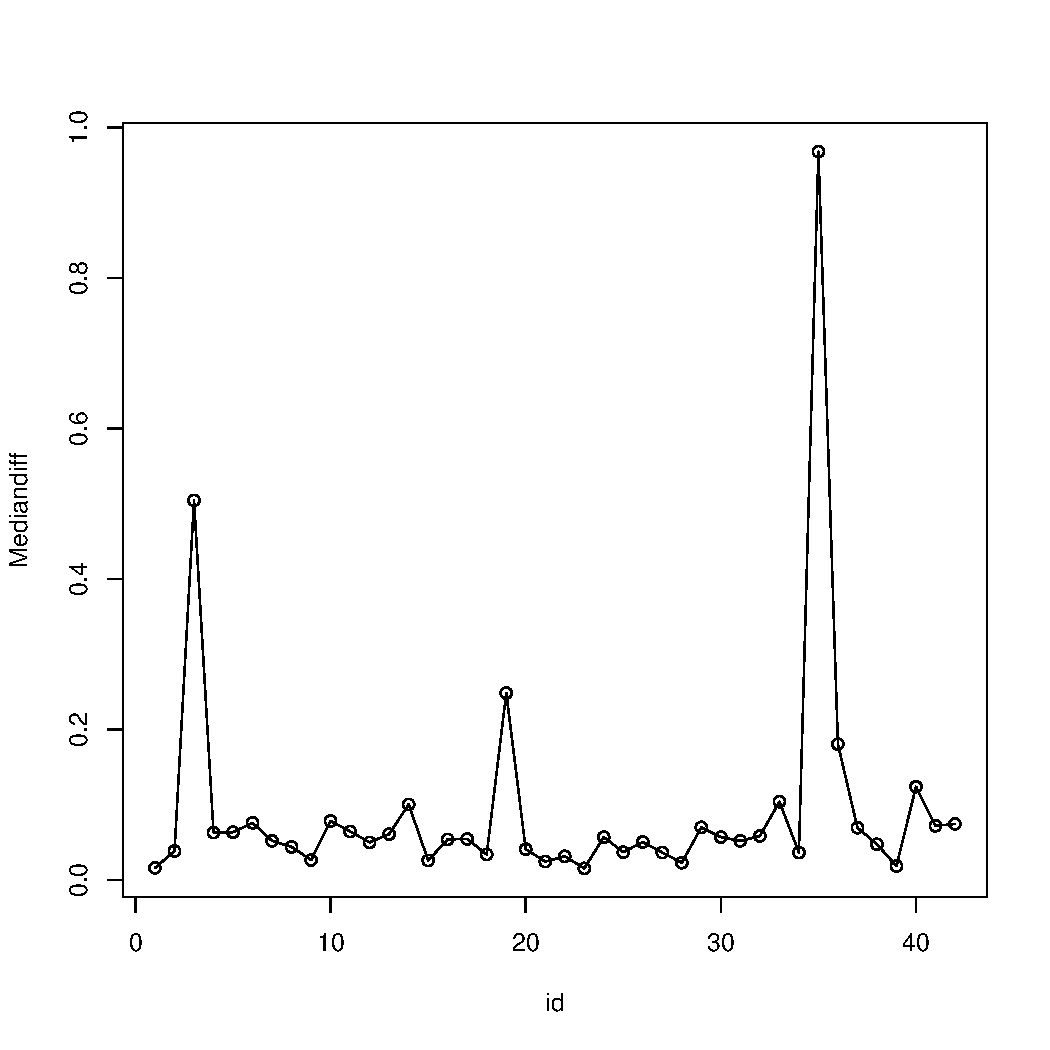
\includegraphics[scale=0.5]{Figures/evolution.pdf}
    \caption{The evolution of the impact of an option on performance.}
    \label{fig:evolution}
\end{figure}


The goal of this research question is to better understand when a configuration option shows a pick in the performance degradation. Such a findings can indicate development patterns that lead to a performance degradation. For example, Figure~\ref{fig:evolution} shows the impact of an option on the performance. Basically, that option has no impact on the performance except on two versions, so it will be interesting to see what happens on these two commits. 

RQ3: \RQIII

An option can suddenly show a pick in the performance, the goal of this research question is to better understand when developers fix that pick: is it immediately, after a while, in the same release, or in next release, .... This research question can also study how developers fix that performance regression. Figure~\ref{fig:evolution} shows that developers fixed that two performance regression immediately.   


\section{Related Work}

https://arxiv.org/abs/1710.07980:
\begin{itemize}
    \item "We built a testing scaffold for the 26,000+ configurations of JHipster using a cluster of 80 machines during 4 nights for a total of 4,376 hours (182 days) CPU time"
\end{itemize}



\bibliographystyle{IEEEtran}
\bibliography{ConfigSLR}


\end{document}
